\documentclass{tstextbook}

\begin{document}

\tsbook{Projet Tatamis}
       {ANGER Benoit - BOURGINE Bruno}
       {Utagawa Hiroshige / Carrie May}
       {2021-2022}
       {xxxxx}{xxx--xx--xxxx--xx--x}{0.1}
       {}
       {}

%---------------------------------------------------------------------------
% Chapters
%---------------------------------------------------------------------------

%---------------------------------------------------------------------------

\chapter{Présentation}
\begin{summary}
    Ce premier chapitre sera l'occasion d'introduire le projet tel qu'il a été initié et de 
    détailler les outils et les méthodes envisagées pour son développement.
  \end{summary}

\section{Descriptif de la problématique}


Le pavage du plan avec des rectangle est un problème classique et déjà largement documenté,
mais je souhaite l'aborder par un aspect très concret : étant donné un nombre de tatamis, quelles sont les
configurations possibles.\\
\begin{center}
    \includegraphics[width = 0.5\linewidth]{./images/pavage-par-tatamis.png}
\end{center}
C'est un problème que rencontre notamment toute personne qui se retrouve à devoir installer un dojo.
Il existe une contrainte de base qui est que 4 tatamis ne rejoignent jamais en un même coin. Mais ont peut
en ajouter d'autres : possibilité de demi-tatamis (carré), répartition des couleurs, répartition de l'usure...

\section{Ébauche de cahier des charges}

Utilisateur final : gestionnaire de dojo\\

L'interface utilisateur devra comprendre un menu de paramétrage basique : nombre de tatamis,
contraintes géométriques, contraintes d'aspect général; ainsi qu'un affichage des dispositions envisageables.\\

L'utilisateur devra pouvoir saisir :

\begin{itemize}
    \item le nombre et le type (entier/demis) de tatamis à disposition
    \item leurs dimensions
    \item leurs couleurs
    \item éventuellement leur état (on dispose de préférence les plus usés en périphérie)
    \item les dimensions du dojo
\end{itemize}

L'affichage proposera différentes disposition selon les contraintes imposées.

\section{Membres du projet}


\chapter{Cahier des charges}
\section{Démarche}

La problématique initiale telle qu'elle a été énoncée est la suivante : \emph{étant donné un nombre de tatamis, quelles sont les 
configurations possibles ?}\\

Les dojos sont de dimension m (longueur) x n (largeur) unités. Et les tatamis sont de dimension 1 x 2 unités. Il existe parfois des demi-tatamis de dimension 1 x 1 unité.
Pour disposer les tatamis, il existe une contrainte: quatre coins de tatamis ne peuvent pas se retrouver en un même point.

Nous allons ici détaillé plus précisément le cahier des charges de l'application. Nous listerons les \emph{epics} afin d'en déduire
les \emph{users stories} et leurs tâches afférentes, et ainsi établir la \emph{roadmap} de notre projet. Le cahier des charges est formulé 
du point de vue de l'utilisateur final, les \emph{epics} étant rédigées sous la forme : \emph{en tant que} \dots ,\emph{je souhaite} \dots ,\emph{afin de } \dots.\\


Par ailleurs afin de prioriser les demandes, nous classerons les fonctionnalités en deux catégories :

\begin{itemize}
    \item essentielles (must have)
    \item optionnelles (nice to have)
\end{itemize}

\section{Persona de l’utilisateur final}

L’utilisateur final est un gestionnaire de dojo.\\

A propos:
\begin{itemize}
    \item Les gestionnaires de dojo ont des profils et backgrounds variés. Il peut être très avancé 
    ou très novice en informatique et en géométrie
    \item En revanche, avec un peu de formation et si on lui installe les outils, il sera capable 
    des les utiliser même si l’ergonomie n’est pas idéale
\end{itemize}


Objectifs:
\begin{itemize}
    \item Préparer le dojo pour qu’il soit prêt pour les entraînements et compétitions
    \item Assurer l’usure équitable des tatamis par des modifications régulières de disposition
\end{itemize}

Points de douleur:
\begin{itemize}
    \item Quand il arrive sur un nouveau dojo, il est difficile de savoir rapidement si une 
    combinaison de tatamis est possible ou non
    \item Il est également difficile de savoir combien de tatamis lui sont nécessaires pour 
    faire le dojo
    \item A chaque fois qu’il faut nettoyer le dojo, il faut enlever tous les tatamis, et 
    il est compliqué de refaire le dojo
    \item En particulier lorsqu’il a des demi-tatamis ou des tatamis de couleurs différentes

\end{itemize}



\section{Fonctionnalités essentielles}

%\item \emph{En tant que } gestionnaire de dojo,\emph{ je souhaite} ... \emph{ afin de }...

\begin{itemize}
    \item En tant que gestionnaire de dojo, je souhaite savoir s’il existe une solution pour
     un dojo d'une dimension donnée, afin de savoir si je pourrais remplir mon dojo ou non.
\end{itemize}


\textbf{ Si une solution existe :}

\begin{itemize}
    \item \emph{En tant que} gestionnaire de dojo, 
    \emph{ je souhaite} connaître le nombre de tatamis nécessaires pour un dojo d'une dimension donnée,
    \emph{afin de } n’en déployer que le nombre nécessaire.
    \item \emph{En tant que} gestionnaire de dojo,
    \emph{ je souhaite} connaître le nombre de dispositions possibles pour un dojo d'une dimension donnée, 
    \emph{ afin d'}anticiper la complexité du placement des tatamis.
    \item \emph{En tant que} gestionnaire de dojo ,
    \emph{ je souhaite} visualiser l'ensemble des dispositions possibles, pour un dojo d'une dimension donnée
    \emph{afin de } m’aider à placer les tatamis sur mon dojo.
    \item \emph{En tant que} gestionnaire de dojo, 
    \emph{ je souhaite} pouvoir renseigner le nombre de tatamis dont je dispose, 
    \emph{afin d'}obtenir une solution adaptée à mon matériel.
    \item \emph{En tant que} gestionnaire de dojo,
    \emph{ je souhaite} voir afficher les dimensions (longueur, largeur, surface) des dispositions proposées  
    \emph{ afin d' }exploiter aux mieux l'espace disponible à l'intérieur et à l'extérieur du tatamis.
\end{itemize}


\section{Fonctionnalités optionnelles}


\begin{itemize}
    \item \emph{En tant que} gestionnaire de dojo, 
    \emph{ je souhaite} connaître le nombre de dispositions possibles, modulo une rotation ou une symétrie 
    \emph{ afin de } ne voir sur l’écran que les solutions réellement différentes.
    \item \emph{En tant que} gestionnaire de dojo, 
    \emph{ je souhaite} visualiser l’ensemble des dispositions possibles, modulo une rotation ou une symétrie 
    \emph{ afin de } ne voir sur l’écran que les solutions réellement différentes.
    % \item \emph{En tant que } gestionnaire de dojo,
    % \emph{ je souhaite} je souhaite savoir s'il est utile d’utiliser des demi-tatamis
    % \emph{ afin de } trouver une solution quand elle n’existe pas sans demi-tatamis.
    % \item \emph{En tant que } gestionnaire de dojo,
    % \emph{ je souhaite} avoir visuellement les dispositions possibles en utilisant un nombre donné de demi-tatamis
    % \emph{ afin de } pouvoir exploiter tous les demi-tatamis dont je dispose. 
    \item \emph{En tant que } gestionnaire de dojo,
    \emph{ je souhaite} pouvoir modifier les dimensions d'un tatamis
     \emph{ afin de } obtenir des propositions correspondant à mon matériel.
    \item \emph{En tant que } gestionnaire de dojo,
    \emph{ je souhaite} pouvoir créer des catégories de couleurs de tatamis
     \emph{ afin de } visualiser des propositions de placement avec les couleurs réelles.
    % \item \emph{En tant que } gestionnaire de dojo,
    % \emph{ je souhaite} pouvoir renseigner des critères de placement (par exemple une symétrie, un motif particulier…) 
    % \emph{ afin de } disposer de la meilleure solution selon moi.
\end{itemize}

\chapter{Méthodologie}
\section{Choix de méthodologie}

La méthodologie agile nous paraît très adaptée au développement de notre programme.
En effet, la méthodologie agile:

\begin{itemize}
    \item  Est particulièrement adaptée à la résolution de problème complexes
          et incertaines ou l’on ne sait pas forcément avec précisions l’objectif
          final ou la manière d’y arriver, ce qui est notre cas
    \item Est basée sur l'itération avec la production de livrables testables
          à la fin de chaque \emph{sprint}, ce qui semble adapté pour produire nos différentes
          versions (alpha, beta…)
    \item Est basée sur une équipe multidisciplinaire qui couvre toutes les compétences
          pour produire un produit fini et qui s’auto organise, ce qui parait également
          adapté à notre contexte
\end{itemize}

La méthodologie agile, étant particulièrement adaptée aux situations d'incertitude, préconise
une planification au fur et à mesure de temps, plutôt que d’importantes et lourdes activités de planification en début de projet car les informations manquent pour cette planification totale en amont.

Pour nous donner un cadre, nous nous inspirons très fortement du schéma “Scrum” et du guide Scrum1, tout en l’adaptant à notre situation présente avec des ressources limitées et des contraintes particulières.

\section{Les événements}

\subsection{Les sprints et les phases du projet}


Les sprints sont des périodes de développement ayant un objectif précis et permettant d'arriver à une version du programme. 
Compte tenu du planning imposé par l’exercice, les sprints seront de durée variable et d'une durée légèrement supérieur à un mois (contrairement à ce qui est suggéré par le schéma Scrum).
Les sprints commencent par la session de planning et se terminent par la revue et la rétrospective (événements détaillés ci-après). Elles comprennent également des activités de 'raffinement' ou de préparation du prochain sprint, pour qu’un nouveau sprint puisse commencer immédiatement après la clôture du précédent sprint.
Quatre sprints sont programmés pour le projet aboutissant aux versions Alpha, Beta, Release Candidate et Production.

Nb: Une phase additionnelle de pré-développement aura lieu en amont pour la préparation du projet, mais est organisée de manière ad-hoc et ne peut être considérée comme un sprint. Cette phase a pour objectif d’analyser la demande (le cahier des charges), de déterminer la méthodologie et gouvernance et de préparer le développement pour aboutir sur une roadmap, un plan de développement global du programme qui sera bien sûr affiné au cours du temps.

\subsection{La session de planning du sprint}

Pour chaque sprint la session de planning permet de déterminer:

\begin{itemize}
    \item Le ‘Quoi’: quels éléments du backlog global peuvent être embarqué dans ce sprint pour créer le Sprint backlog
    \item Le ‘Comment’: comment chaque élément du Sprint backlog seront techniquement traités
    \item Le ‘Pourquoi’: quel objectif pour le sprint, sachant que chaque sprint doit délivrer un produit qui peut être limité en fonctionnalités mais qui fonctionne
\end{itemize}

Les décisions sont prises de la manière suivante:
 Quoi et pourquoi
Les propositions d'éléments à ajouter et d’objectif du sprint viennent du product owner. L'équipe de développement prend ensuite la décision de manière souveraine et autonome en session de planification.

\chapter{Choix des outils et langages}
\section{Outils de communications}

\subsection{Redmine}

Cet outil de gestion de projet a été choisi en premier lieu pour sa disponibilité immédiate (il n'y a pas eu d'installation
ou de paramétrage de serveur à réaliser) mais aussi pour sa complétude en terme d'outils. Il dispose
en effet de l'ensemble des fonctionnalités dont nous avions besoin pour ce qui est de la création, de l'ordonnancement
et du suivi des demandes. En cela il est tout à fait adapté à la méthodologie choisie.\\

Nous avons pu le paramétrer un peu plus finement de façon à ce que les caractéristiques et l'évolution des demandes
correspondent à la terminologie employée pour détailler notre projet : type de tracker, statut des demandes, champs personnalisés\dots


\subsection{Slack}

Slack a été choisi comme outil de communication entre les membres de l'équipe afin d'établir des canaux de discussion différenciés. 
Cela permet à l'équipe des échanges plus ciblés et donc plus efficaces, ainsi qu'une vision plus ordonnée de l'historique des communications.

\subsection{Github}

La plateforme Github a été choisie pour héberger et gérer l'ensemble des éléments du projet, à savoir
le code de l'application ainsi que le rapport.

Le dépot est consultable à l'adresse : \url{https://github.com/bubobou/tatamis}

\section{Développement}

\subsection{Langage}

De part sa facilité d'assimilation et les nombreuses bibliothèques disponibles, le choix du langage de programmation
s'est porté sur Python dans sa version 3.9.

\subsection{Bibliothèques}

Différentes bibliothèques nous ont parues d'emblée utiles pour aborder ce projet. Tout d'abord
une recherche documentaire nous a menée vers la bibliothèque \textsf{facile} permettant de traiter
de la programmation par contrainte. Même s'il ne sera pas forcément retenue dans la version finale, 
sa disponibilité nous permet d'aborder plus sereinement notre problématique.\\

Par ailleurs dans la finalité d'une application avec interface graphique, potentiellement portée sur terminal mobile,
 nous avons envisagé l'utilisation de bibliothèques et d'utilitaires tels que :

 \begin{itemize}
     \item \textsf{PyQt}
     \item \textsf{Kivy}
     \item \textsf{python for android}
 \end{itemize}


\chapter{Roadmap globale}
\section{Roadmap au 08/01/2022}

\subsection{Éléments}

\noindent%
\includegraphics[scale=0.5]{images/prepa.png}

\noindent%
\includegraphics[scale=0.5]{images/roadmap_alpha.png}\\
\includegraphics[scale=0.5]{images/roadmap_beta.png}\\
\includegraphics[scale=0.5]{images/roadmap_RC.png}\\
\includegraphics[scale=0.5]{images/roadmap_prod.png}

\subsection{Gantt}

\noindent%
\includegraphics[scale=0.5]{images/Gantt0801.png}


\chapter{Version Alpha}
\section{Backlog/roadmap du sprint Alpha}

L’objectif de ce sprint est de poser les fondations et délivrer les fonctionnalités de bases attendues par l’utilisateur, 
c'est-à- dire la compréhension des dispositions possibles et impossibles.

Pour ce faire le backlog suivant a été "embarqué" dans cette version et a résulté en la roadmap suivante:

%TODO insérer roadmap

\section{Tests}


\noindent%
\begin{adjustwidth}{-1.5cm}{0cm}

    \renewcommand{\arraystretch}{1.2}
    {\setlength{\tabcolsep}{1.5 mm}
        \begin{testtabular}{|m{0.6cm}|m{5.5cm}|m{8cm}|m{2cm}|c|} \hline
            id                                                                             & Sujet                                                                                & Test d'acceptance                                                                                        & Méthode de test & Résultat \\ \hline
            518                                                                            & TACHE Utiliser la fonction pour renvoyer la réponse au gestionnaire de dojo          &
            Quand le programme est lancé et que l'utilisateur saisi comme attendu,
            une réponse lui est renvoyée dans la console                                   & Manuel                                                                               & OK                                                                                                                                    \\ \hline
            517                                                                            & TACHE Créer une fonction permettant de calculer le nombre de tatamis nécessaires
            étant donné des dimensions de dojo et qu'une solution existe                   &
            Quand la fonction est exécutée, elle retourne le nombre de tatamis nécessaires &
            Automatisé                                                                     & OK                                                                                                                                                                                                                           \\ \hline
            \multirow{3}{0.6cm}{516}                                                       & \multirow{3}{5.5cm}{TACHE Permettre au gestionnaire de dojo de poser cette question} & 1. Quand le programme est lancé, il demande a l'utilisateur la largeur du dojo                           & Automatisé      & OK       \\ \cline{3-5}
                                                                                           &                                                                                      & 2. Quand le programme est lancé, il demande a l'utilisateur la longueur du dojo                          & Automatisé      & OK       \\ \cline{3-5}
                                                                                           &                                                                                      & 3. Quand le programme est lancé, une option est disponible pour l'utilisateur pour poser cette question. & Automatisé      & OK       \\ \hline
        \end{testtabular}}
\end{adjustwidth}


\noindent%
\begin{adjustwidth}{-1.5cm}{0cm}

    \renewcommand{\arraystretch}{1.2}
    {\setlength{\tabcolsep}{1.5 mm}
        \begin{testtabular}{|m{0.6cm}|m{5.5cm}|m{8cm}|m{2cm}|c|} \hline
            id                       & Sujet                                                                                                                                         & Test d'acceptance                                                                                                                                                                                                          & Méthode de test & Résultat \\ \hline
            515                      & TACHE Créer une fonction permettant de calculer le nombre de tatamis nécessaires étant donné des dimensions de dojo et qu'une solution existe & Quand la fonction est executée, elle retourne le nombre de tatamis nécessaires                                                                                                                                             & Automatisé      & OK       \\ \hline

            \multirow{3}{0.6cm}{514} & \multirow{3}{5.5cm}{TACHE Permettre au gestionnaire de dojo de poser cette question}                                                          & 1. Quand le programme est lancé, il demande à l'utilisateur la largeur du dojo                                                                                                                                             & Automatisé      & OK       \\ \cline{3-5}
                                     &                                                                                                                                               & 2. Quand le programme est lancé, il demande à l'utilisateur la longueur du dojo                                                                                                                                            & Automatisé      & OK       \\ \cline{3-5}
                                     &                                                                                                                                               & 3. Quand le programme est lancé, une option est disponible pour l'utilisateur pour poser cette question.                                                                                                                   & Automatisé      & OK       \\ \hline
            \multirow{2}{0.6cm}{513} & \multirow{2}{5.5cm}{US Comprendre le nombre de dispositions possibles}                                                                        & \cellcolor{tsgrey} 1. Étant donné que l'utilisateur saisie des dimensions de dojo, quand il saisie 2, il obtient le nombre conformément à l'article de Ruskey et Woodcock de 2009                                        & Automatisé      & OK       \\ \cline{3-5}
                                     &                                                                                                                                               & \cellcolor{tsgrey} 2. Étant donné que l'utilisateur saisie des dimensions de dojo en inversant la longueur et la largeur, quand il saisie 2, il obtient le nombre conformement a l'article de Ruskey et Woodcock de 2009 & Automatisé      & OK       \\ \hline

            512                      & TACHE Utiliser la fonction pour renvoyer la réponse au gestionnaire de dojo	Alpha                                                              & Quand le programme est lancé et que l'utilisateur saisie comme attendu, une réponse lui est renvoyée dans la console                                                                                                       & Automatisé      & OK       \\ \hline
            \multirow{2}{0.6cm}{511} & \multirow{2}{5.5cm}{TACHE Demander les dimensions et permettre au gestionnaire de dojo de les saisir}                                         & 1. Quand le programme est lancée, il demande a l'utilisateur la largeur du dojo                                                                                                                                            & Automatisé      & OK       \\ \cline{3-5}
                                     &                                                                                                                                               & 2. Quand le programme est lancé, il demande a l'utilisateur la longueur du dojo                                                                                                                                            & Automatisé      & OK       \\ \hline
            \multirow{2}{0.6cm}{510} & \multirow{2}{5.5cm}{US Comprendre si une solution existe}                                                                                     & \cellcolor{tsgrey} 1. Etant donné que l'utilisateur saisie des dimensions de dojo n'ayant pas de solution, quand il saisie 1, il obtient 'Il n'existe pas de disposition possible avec des tatamis 2x1 pour ce dojo'     & Automatisé      & OK       \\ \cline{3-5}
                                     &                                                                                                                                               & \cellcolor{tsgrey} 2. Étant donné que l'utilisateur saisie des dimensions de dojo ayant au moins une disposition, quand il saisie 1, il obtient 'Il existe au moins une disposition avec des tatamis 2x1 pour ce dojo'   & Automatisé      & OK       \\ \hline
        \end{testtabular}}
\end{adjustwidth}


\noindent%
\begin{adjustwidth}{-1.5cm}{0cm}

    \renewcommand{\arraystretch}{1.2}
    {\setlength{\tabcolsep}{1.5 mm}
        \begin{testtabular}{|m{0.6cm}|m{5.5cm}|m{8cm}|m{2cm}|c|} \hline
            id                                                                                                       & Sujet                                                                                                                                  & Test d'acceptance                                                                                                                                                                  & Méthode de test & Résultat \\ \hline
            \multirow{2}{0.6cm}{509}                                                                                 & \multirow{2}{5.5cm}{US Créer la fonction permettant de calculer le nombre de solutions au problème étant donné les dimensions du dojo} & 1. Quand la fonction est exécutée, elle retourne le nombre de dispositions possibles conformément a l'article de Ruskey et Woodcock de 2009                                        & Automatisé      & OK       \\ \cline{3-5}
                                                                                                                     &                                                                                                                                        & 2. Quand la fonction est exécutée en inversant la longueur et la largeur, elle retourne le nombre de dispositions possibles conformément a l'article de Ruskey et Woodcock de 2009 & Automatisé      & OK       \\ \hline

            509                                                                                                      & EPIC Développer pour un gestionnaire de dojo un outil simple lui permettant de saisir les dimensions du dojo et
            de savoir si un solution existe, le nombre de tatamis nécessaires et le nombre de dispositions possibles & \cellcolor{tsgrey} cf. tests utilisateurs des US                                                                                     &                                                                                                                                                                                    &                            \\ \hline
            \multirow{2}{0.6cm}{480}                                                                                 & \multirow{2}{5.5cm}{US Calculer le nombre de tatamis nécessaires}                                                                      & 1. Étant donne que l'utilisateur saisit des dimensions de dojo avec une solution qui existe, quand il saisie 3, il obtient le nombre de tatamis nécessaires                        & Automatisé      & OK       \\ \cline{3-5}
                                                                                                                     &                                                                                                                                        & 2. Étant donne que l'utilisateur saisit des dimensions de dojo avec aucune disposition possible, quand il saisie 3, il obtient un message indiquant l'absence de solution          & Automatisé      & OK       \\ \hline
        \end{testtabular}}
\end{adjustwidth}



\bigskip

Les tests automatisés sont définis dans le fichier \texttt{test\_alpha.py} et \texttt{test\_interface.py}. Ils peuvent être reproduits 
en l'exécutant avec ligne de commande \texttt{python3 -m pytest}.


\section{Documentation utilisateur Alpha}

\subsection{Prérequis}
%TODO faire mise en page
Configuration et installations requises:

\begin{itemize}
    \item Python 3.9 ou supérieur
    \item Librairies Python: aucune
\end{itemize}

\subsection{Comment trouver le nombre de tatamis nécessaires pour remplir un dojo?}

Lancer le programme dans un Terminal (ligne de commande: python3 interface.py)
Entrer (dans le Terminal) la longueur et la largeur du dojo en suivant les questions posées par le programme. Nb: Vous pouvez inverser la longueur et la largeur, cela n’a pas d’importance
Répondre ‘3’ à la question du programme “Que cherchez vous?”
Interpréter la réponse:
Réponse : “Le nombre de tatamis 2x1 nécessaires pour ce dojo est : [Nombre]”. Interprétation: il existe au moins une disposition possible et vous aurez besoin d’exactement [Nombre] tatamis pour remplir le dojo.
Réponse : “Il n'existe pas de disposition possible avec des tatamis 2x1 pour ce dojo”. Interprétation: il n’existe aucune disposition possible de tatamis 2 x 1 pour remplir le dojo.

\subsection{Comment savoir s’il existe une disposition possible de tatamis pour un dojo donné?}

Lancer le programme dans un Terminal (ligne de commande: python3 interface.py)
Entrer (dans le Terminal) la longueur et la largeur du dojo en suivant les questions posées par le programme. Nb: Vous pouvez inverser la longueur et la largeur, cela n’a pas d’importance
Répondre ‘1’ à la question du programme “Que cherchez vous?”
Interpréter la réponse:
Réponse : “Il existe au moins une disposition avec des tatamis 2x1 pour ce dojo”. Interprétation: il existe au moins une disposition possible.
Réponse : “Il n’existe pas de disposition possible avec des tatamis 2x1 pour ce dojo”. Interprétation: il n’existe aucune disposition possible de tatamis 2 x 1 pour remplir le dojo. Il est dans ce cas probable de devoir utiliser des demi-tatamis pour remplir pleinement le dojo.


\subsection{Comment savoir combien il existe de dispositions possibles de tatamis pour un dojo donné?}

Lancer le programme dans un Terminal (ligne de commande: python3 interface.py)
Entrer (dans le Terminal) la longueur et la largeur du dojo en suivant les questions posées par le programme. Nb: Vous pouvez inverser la longueur et la largeur, cela n’a pas d’importance
Répondre ‘2’ à la question du programme “Que cherchez vous?”
Interpréter la réponse:
a. Réponse : “Il existe [Nombre] dispositions possibles”. Interprétation: des dispositions existent pour ce dojo et il y en a [Nombre].
b. Réponse : “Il existe 0 disposition possible”. Interprétation: il n’existe pas de disposition pour ce dojo.


\section{Explication des algorithmes et choix de programmation}

\subsection{Algorithme pour les calculs de nombre de dispositions}

Nous avons tenté deux approches pour répondre à ces fonctionnalités de base:
1. Exploitation de la bibliothèque facile écrite en python pour résoudre des problèmes en programmation par contrainte. 
La publication de Xavier Olive (ref) proposant une application de cette  bibliothèque au problème qui nous concerne, 
nous avons explorer la possibilité d’adapter le programme proposé dans la publication. Si le nombre de dispositions 
proposées lors des calculs pour des dimensions de dojo données est tout à fait cohérent avec les valeurs trouvées 
dans les autres publications traitant de ce problème, il nous est rapidement apparu que les dimensions étaient limités, 
et que le temps de calcul n’était pas satisfaisant.

2. Application de l’approche proposée par Dean Hickerson (Filling rectangular rooms with Tatami mats, 2002): %TODO ajouter note bas de page
nous avons codé le programme mathématique qu’il décrit en python.

La méthode 2 a finalement été retenue car elle a l’avantage d'être très légère et rapide en exécution. 
Elle peut notamment calculer rapidement des réponses même si les dimensions sont grandes (nous n’avons d’ailleurs par 
limites les dimensions saisies a un certain nombre).


\subsection{Choix de programmation Interface}

Pour faire à l'essentiel, il a été choisi d'utiliser le terminal pour les interactions entre l'utilisateur et le programme. 
Ce n’est évidemment pas idéal, mais cela a permis de rapidement traiter la partie interface pour se concentrer sur 
les fonctionnalités et les calculs mathématiques permettant d’y répondre.

\subsection{Choix de la structure du programme}

Il nous semble important de suivre et mettre en application des principes SOLID, et en particulier du 
‘Single Responsibility Principle’ et ‘Open-Closed Principle’. 
A ce stade, vu la simplicité du programme, ce n’est pas forcément nécessaire ni applicable de manière évidente, 
mais nous souhaitons construire des fondations solides pour la suite:
Un fichier a une fonction principale
Dans cette version alpha, nous avons 2 fichiers (un fichier de front-end interface.py et un fichier de back-end alpha.py) :
interface.py : fichier contient toutes les fonctionnalités de front-end, c’est à dire l’interface utilisateur
alpha.py : fichier qui reprend les fonctions de calculs (basiques) de back-end


\section{Challenges rencontrés et apprentissage}

\subsection{Challenges rencontrés et solutions appliquées}

Les deux challenges principaux de cette version ont été les suivants:
Challenges techniques
Bien que pas très exigeante techniquement, cette version pose les fonctionnalités de base sur lesquelles 
les versions suivantes reposent. En ce qui concerne les algorithmes, le challenge principal a été la recherche 
de la documentation qui prend du temps. Mais bien que cela ait demandé du temps, nous avons eu la chance de 
trouver beaucoup de documentation de bonne qualité sur le sujet des tatamis. Il nous a ensuite été relativement 
facile d'implémenter et tester les solutions trouvées.
Challenges organisationnels
Bien que la coopération au sein de l'équipe ait débuté en phase de pré-développement, ce sprint était le premier 
qui impliquait un travail réel sur le code qui pose forcément de nouveaux challenges. Nous avons par ailleurs perdu 
définitivement un membre de l'équipe, impliquant inévitablement plus de travail de la part des membres restants. 
Pour nous permettre de bien avancer, nous avons mis en application les principes organisationnels suivants:
Sessions de travail régulières (hebdomadaires) pour discuter des points ouverts et répartir les tâches. 
Fréquence plutôt élevée pour garder un bon rythme de travail et éviter les accoups.
Retranscription écrite claire des tâches à effectuer avec les dates butoires (et dépendances de tâches lors qu’il y en a) 
avec un Compte Rendu écrit pour chaque session de travail
Communication entre les sessions de travail (par Slack), notamment pour les discussions sur l'exécution des tâches 
pré-requises à d'autres tâches dépendantes.
Travail personnel entre les session pour accomplir les tâches
Par ailleurs, pour gérer le code, github (intégré à Slack pour recevoir les notifications lors des updates) a été utilisé. 

\subsection{Apprentissage}

Les enseignements principaux de ce sprint sont les suivants:
Le choix de méthodologie agile confirmé comme étant la bonne approche pour travailler sur le projet. 
La perte d’un membre de l'équipe aurait notamment été plus difficile à gérer si tout avait été planifié de manière rigide au départ
Le bon fonctionnement de la coopération et organisation choisie (régularité des sessions de travail, documentation des sessions 
de travail avec des tâches et dates butoires claires,...)


\chapter{Version Beta}
\section{Backlog/roadmap du sprint Beta}

L’objectif de ce sprint est de donner bien plus de valeur à l'utilisateur par:
\begin{enumerate}
    \item Une visualisation des dispositions possible (ce qui apporte bien plus à l'utilisateur que la version Alpha)
    \item Une utilisation facilité par une interface utilisateur intuitive et facile
\end{enumerate}

Pour ce faire le backlog suivant a été "embarqué" dans cette version et a résulté en la roadmap suivante:


\section{Tests}


\noindent%
\begin{adjustwidth}{-1.5cm}{0cm}

    \renewcommand{\arraystretch}{1.2}
    {\setlength{\tabcolsep}{1.5 mm}
    
        \begin{testtabular}{|m{0.6cm}|m{5.5cm}|m{8cm}|m{2cm}|c|} \hline
            id                       & Sujet                                                                   & Test d'acceptance                                                                                             & Méthode de test & Résultat \\ \hline
            \multirow{2}{0.6cm}{539} & \multirow{2}{5.5cm}{TACHE Cliquer pour avoir accès aux fonctionnalités} & Quand l'application est lancée, les boutons s'affichent                                                       & Manuel          & OK       \\ \cline{3-5}
                                     &                                                                         & Quand l'utilisateur clique sur un bouton, la fonctionnalité est activée.                                      & Manuel          & OK       \\ \hline
            \multirow{3}{0.6cm}{538} & \multirow{3}{5.5cm}{TACHE Valider les dimensions}                       & Quand l'application est lancée, seules des valeurs entières peuvent être entrées                              & Manuel          & OK       \\ \cline{3-5}
                                     &                                                                         & Quand l'application est lancée, les valeurs entrables sont restreintes aux valeurs dans un intervalle défini. & Manuel          & OK       \\ \cline{3-5}
                                     &                                                                         & Quand l'utilisateur omet ou entre 0 pour au moins une dimension, un message d'erreur s'affiche.               & Manuel          & OK       \\ \hline
        \end{testtabular}}
\end{adjustwidth}


\noindent%
\begin{adjustwidth}{-1.5cm}{0cm}

    \renewcommand{\arraystretch}{1.2}
    {\setlength{\tabcolsep}{1.5 mm}
        
            \begin{testtabular}{|m{0.6cm}|m{5.5cm}|m{8cm}|m{2cm}|c|} \hline
                id                       & Sujet                                                                                           & Test d'acceptance                                                                                                                                                & Méthode de test & Résultat \\ \hline
                537                      & TACHE Offrir la possibilité d'entrer des dimensions de dojo                                     & Quand l'application est lancée, une fenêtre s'ouvre avec la possibilité d'entrer les dimensions.                                                                 & Manuel          & OK       \\ \hline
                536                      & TACHE Créer la fonction permettant d'afficher toutes les solutions                              & Quand la fonction reçoit en input les coordonnées des tatamis pour une disposition dimensions, alors elle retourne un graph avec toutes les solutions possibles" & Manuel          & OK       \\ \hline
                535                      & TACHE Créer la fonction permettant d'afficher une seule solution                                & Quand la fonction reçoit en input les coordonnées des tatamis pour une disposition dimensions, alors elle retourne un graph avec une solution possible"          & Manuel          & OK       \\ \hline
                534                      & TACHE Créer la fonction permettant de calculer les coordonnées des tatamis pour une disposition & Quand la fonction reçoit en input les dimensions d'un dojo, alors elle retourne les coordonnées des tatamis pour une disposition"                                & Manuel          & OK       \\ \hline
                533                      & TACHE Créer la fonction permettant de choisir d'afficher toutes les solutions                   & Étant donné les inputs des dimensions d'un dojo, quand cette fonction est choisie, elle retourne un graph avec toutes les solutions possibles"                   & Manuel          & OK       \\ \hline
                532                      & US Disposer d'une interface d'affichage ergonomique                                             & Quand le programme est lancé, il ouvre une interface ergonomique"                                                                                                & Manuel          & OK       \\ \hline
                531                      & TACHE Créer une classe de fenêtre type permettant d'avoir un affichage reproductible            & Quand l'application est lancée, une fenêtre s'ouvre avec les bonnes (adaptées à l'écran) et memes dimensions"                                                    & Manuel          & OK       \\ \hline
                530                      & TACHE Créer la fonction permettant de choisir d'afficher une seule solution                     & Étant donné les inputs des dimensions d'un dojo, quand cette fonction est choisie, elle retourne un graph avec une seule solution possible"                      & Manuel          & OK       \\ \hline
                \multirow{2}{0.6cm}{519} & \multirow{2}{5.5cm}{EPIC Permettre au gestionnaire de dojo de visualiser les solutions}         & cf. tests utilisateurs des US                                                                                                                                    &                 & OK       \\ \cline{3-5}
                                         &                                                                                                 & Le nombre de solution du programme donne le meme nombre de solution que le calcul de coordonnées Tatamis                                                         & Automatisé      & OK       \\ \hline
                478                      & US Afficher visuellement toutes les dispositions possibles                                      & Étant donné des dimensions d'un dojo saisies, quand il sélectionne cette option, il obtient visuellement toutes les dispositions possibles"                      & Manuel          & OK       \\ \hline
                476                      & US Afficher visuellement une disposition possible                                               & Étant donné des dimensions d'un dojo saisies, quand il sélectionne cette option, il obtient visuellement une disposition possible"                               & Manuel          & OK       \\ \hline
            \end{testtabular}
    }
\end{adjustwidth}

% Nb: Tests automatisés réalisés avec le fichier “test_beta.py”. Ils peuvent être reproduits en l'exécutant avec ligne de commande “python3 -m pytest”.


\section{Documentation utilisateur Beta}

\subsection{Comment trouver le nombre de tatamis nécessaires?}

\begin{enumerate}
    \item Lancer l’interface (dans le Terminal avec la ligne de commande: python3 interface.py)
    \item Entrer dans l’interface la longueur et la largeur du dojo dans les champs prévus à cet effet.
          \emph{Nb: Vous pouvez inverser la longueur et la largeur, cela n’a pas d’importance}
    \item Cliquer sur le bouton: “Savoir si il existe une disposition pour le dojo”
          \emph{ Nb: Si vous oubliez d’entrer une dimension ou si vous entrez une dimension 0,
              un message d’erreur “Erreur de saisie des dimensions. Aucune dimension ne peut avoir une valeur nulle ou vide” apparaît.}
    \item Interpréter la réponse:
          \begin{enumerate}
              \item  Réponse: “Le nombre de tatamis 2x1 nécessaires pour ce dojo est :
                    [Nombre]”. Interprétation: il existe au moins une disposition possible et vous aurez besoin d’exactement [Nombre] tatamis pour remplir le dojo.
              \item  Réponse: “Le nombre de tatamis 2x1 nécessaires pour ce dojo est :
                    Aucune disposition possible de tatamis 2x1 pour ce dojo”. Interprétation:
                    il n’existe aucune disposition possible de tatamis 2 x 1 pour remplir le dojo.
          \end{enumerate}
\end{enumerate}

\subsection{Comment savoir s’il existe une disposition possible de tatamis pour un dojo donné?}

\begin{enumerate}
    \item Lancer l’interface (dans le Terminal avec la ligne de commande: python3 interface.py)
    \item Entrer dans l’interface la longueur et la largeur du dojo dans les champs prévus à cet effet.
          \emph{Nb: Vous pouvez inverser la longueur et la largeur, cela n’a pas d’importance}.
    \item Cliquer sur le bouton: “Connaître le nombre de dispositions possibles” \emph{Nb: Si vous oubliez d’entrer une dimension ou
              si vous entrez une dimension 0, un message d’erreur “Erreur de saisie des dimensions.
              Aucune dimension ne peut avoir une valeur nulle ou vide” apparaît.}
    \item Interpréter la réponse:
          \begin{enumerate}
              \item     Réponse: “Il existe au moins une disposition avec des tatamis 2x1 pour ce dojo”.
                    Interprétation: il existe au moins une disposition possible.
              \item     Réponse: “Il n’existe pas de disposition possible avec des tatamis 2x1 pour ce dojo”.
                    Interprétation: il n’existe aucune disposition possible de tatamis 2 x 1 pour remplir le dojo.
                    Il est dans ce cas probable de devoir utiliser des demi-tatamis pour remplir pleinement le dojo.
          \end{enumerate}

\end{enumerate}

\subsection{Comment savoir combien il existe de dispositions possibles de tatamis pour un dojo donné?}

\begin{enumerate}
    \item Lancer l’interface (dans le Terminal avec la ligne de commande: python3 interface.py)
    \item Entrer dans l’interface la longueur et la largeur du dojo dans les champs prévus à cet effet. Nb: Vous pouvez inverser la longueur et la largeur, cela n’a pas d’importance
    \item Cliquer sur le bouton: “Connaître le nombre de tatamis 2x1 nécessaires pour la taille du dojo”.
          \emph{Nb: Si vous oubliez d’entrer une dimension ou si vous entrez une dimension 0, un message d’erreur “Erreur de saisie des dimensions. Aucune dimension ne peut avoir une valeur nulle ou vide” apparaît.
          }
    \item Interpréter la réponse:
          \begin{enumerate}
              \item Réponse: “Le nombre de tatamis 2x1 nécessaires pour ce dojo est :  [Nombre] disposition possible”.
                    Interprétation: il faut [Nombre] tatamis pour remplir le dojo.
              \item Réponse: “Il n'existe pas de disposition possible avec des tatamis 2x1 pour ce dojo”.
                    Interprétation: la demande est non pertinente car il n’existe pas de disposition possible de tatamis 2x1 pour les dimensions du dojo.
          \end{enumerate}
\end{enumerate}


\subsection{Comment afficher une disposition?}

\subsection{Comment afficher toutes les dispositions possibles?}

\section{Explication des algorithmes et choix de programmation}

\subsection{Algorithme pour l’affichage des dispositions}

\subsection{Choix de programmation Interface}

Les choix importants concernant l’interface ont été les suivants:


\subsubsection{Choix de la librairie d’interface graphique}

Une recherche initiale a permis d'identifier 5 librairies à notre disposition:

\begin{itemize}
    \item PyQt5
    \item Tkinter
    \item Pyside2
    \item Kivy
    \item wxPython
\end{itemize}

Trois critères de choix ont été appliqués:

\begin{itemize}
    \item Capacités de la librairie
    \item Disponibilité de la documentation et ressources en ligne
    \item Connaissances préalables par l'équipe et simplicité
\end{itemize}

L'évaluation a conclu aux résultats suivants:\\


\noindent%
\begin{adjustwidth}{-1.5cm}{0cm}

    \renewcommand{\arraystretch}{1.2}
    {\setlength{\tabcolsep}{1.5 mm}
               

            \begin{testtabular}{*{6}{|p{0.16\linewidth} }|} \hline                

                \rowcolor{tsgrey}                               &                                                                                                & Tkinter & Pyside2 & Kivy & wxPython \\ \hline
                \cellcolor{lightgray} Capacités de la librairie & Très large variété de widgets (boutons, champs de saisie, boîtes de message…)

                Beaucoup de possibilités

                Grille disponible
                                                                & Large variété de widgets (boutons, champs de saisie, boîtes de message…)

                Grille disponible (mais également une fonctionnalité qui facilite le placement)
                                                                & Large variété de widgets (boutons, champs de saisie, boîtes de message…)

                Grille disponible
                                                                & Widgets disponibles, dont certains bien designés mais d’autres moins intuitifs (par ex. les boutons)

                Grille disponible
                                                                & Large variété de widgets (boutons, champs de saisie, boîtes de message…)

                Grille disponible 
                                                                                                                                                                                  \\ \hline
            \end{testtabular}
        
    }

\end{adjustwidth}

\section{Challenges rencontrés et apprentissage}

\chapter{Version Release Candidate}
\section{Backlog/roadmap du sprint Release}

\chapter{Version Production}
\section{Backlog/roadmap du sprint Production}

L’objectif de ce sprint est de finaliser en augmentant encore la valeur donné à l'utilisateur par: 
Ajout de deux fonctionnalités concernant les dispositions symétriques. L’objectif étant d'éliminer ces dispositions symétriques qui apportent peu, voire prêtent à confusion pour l’utilisateur.
Dernière amélioration mineure de l’interface, surtout sur le visuel, pour aligner le design des messages de réponse à celui de l’interface principale.

Pour ce faire le backlog suivant a été \emph{embarqué} dans cette version et a résulté en la roadmap suivante:

\section{Tests}

Les tests réalisés pour cette version et leurs résultats sont les suivants:

%TODO inclure tableaux tests

Par ailleurs, étant donné qu’il s’agit de la dernière version pour mise en production, 
il est important de tester l’ensemble des fonctionnalités du programme. Des tests de non régression 
ont été effectués:

%TODO inclure tableaux tests non regression

Erreur sur validation des saisies:
Une erreur a été constaté suivant les versions utilisés de PyQt:
\begin{itemize}
    \item Version 5.9.7: la validation de la saisie des données fonctionne (comportement attendu)
    \item Version 5.12.2: la validation fonctionne partiellement (cela limite bien le type d'entrée - uniquement des entiers, et limite le nombre de chiffres, mais cela ne limite pas à 25 ou 300 comme attendu; cela limite uniquement à respectivement 99 et 999). Pour corriger ce changement de comportement de QIntValidator, un nouveau message d’erreur a été mis en place.
\end{itemize}

\section{Documentation Utilisateur Production}

\subsection{Prérequis}

Configuration et installations requises:

\begin{itemize}
    \item Python 3.9 ou supérieur
    \item Librairies Python: datetime, numpy, PyQt5.QtCore, PyQt5.QtGui, PyQt5.QtWidgets, sys, time.
     (Idéalement la version 5.9.7 de PyQt) 
    \item Installer les polices Nexa (light et bold) (fichiers otf fournis)
\end{itemize}


\newpage


% \appendix
% \section{Annexe : version Beta}\label{appendix:beta}

% Arbre des appels récursifs pour la recherche de solutions de pavage d'un dojo de dimension 4 $\times$ 3 

% \begin{adjustwidth}{-1.5cm}{0cm}
% 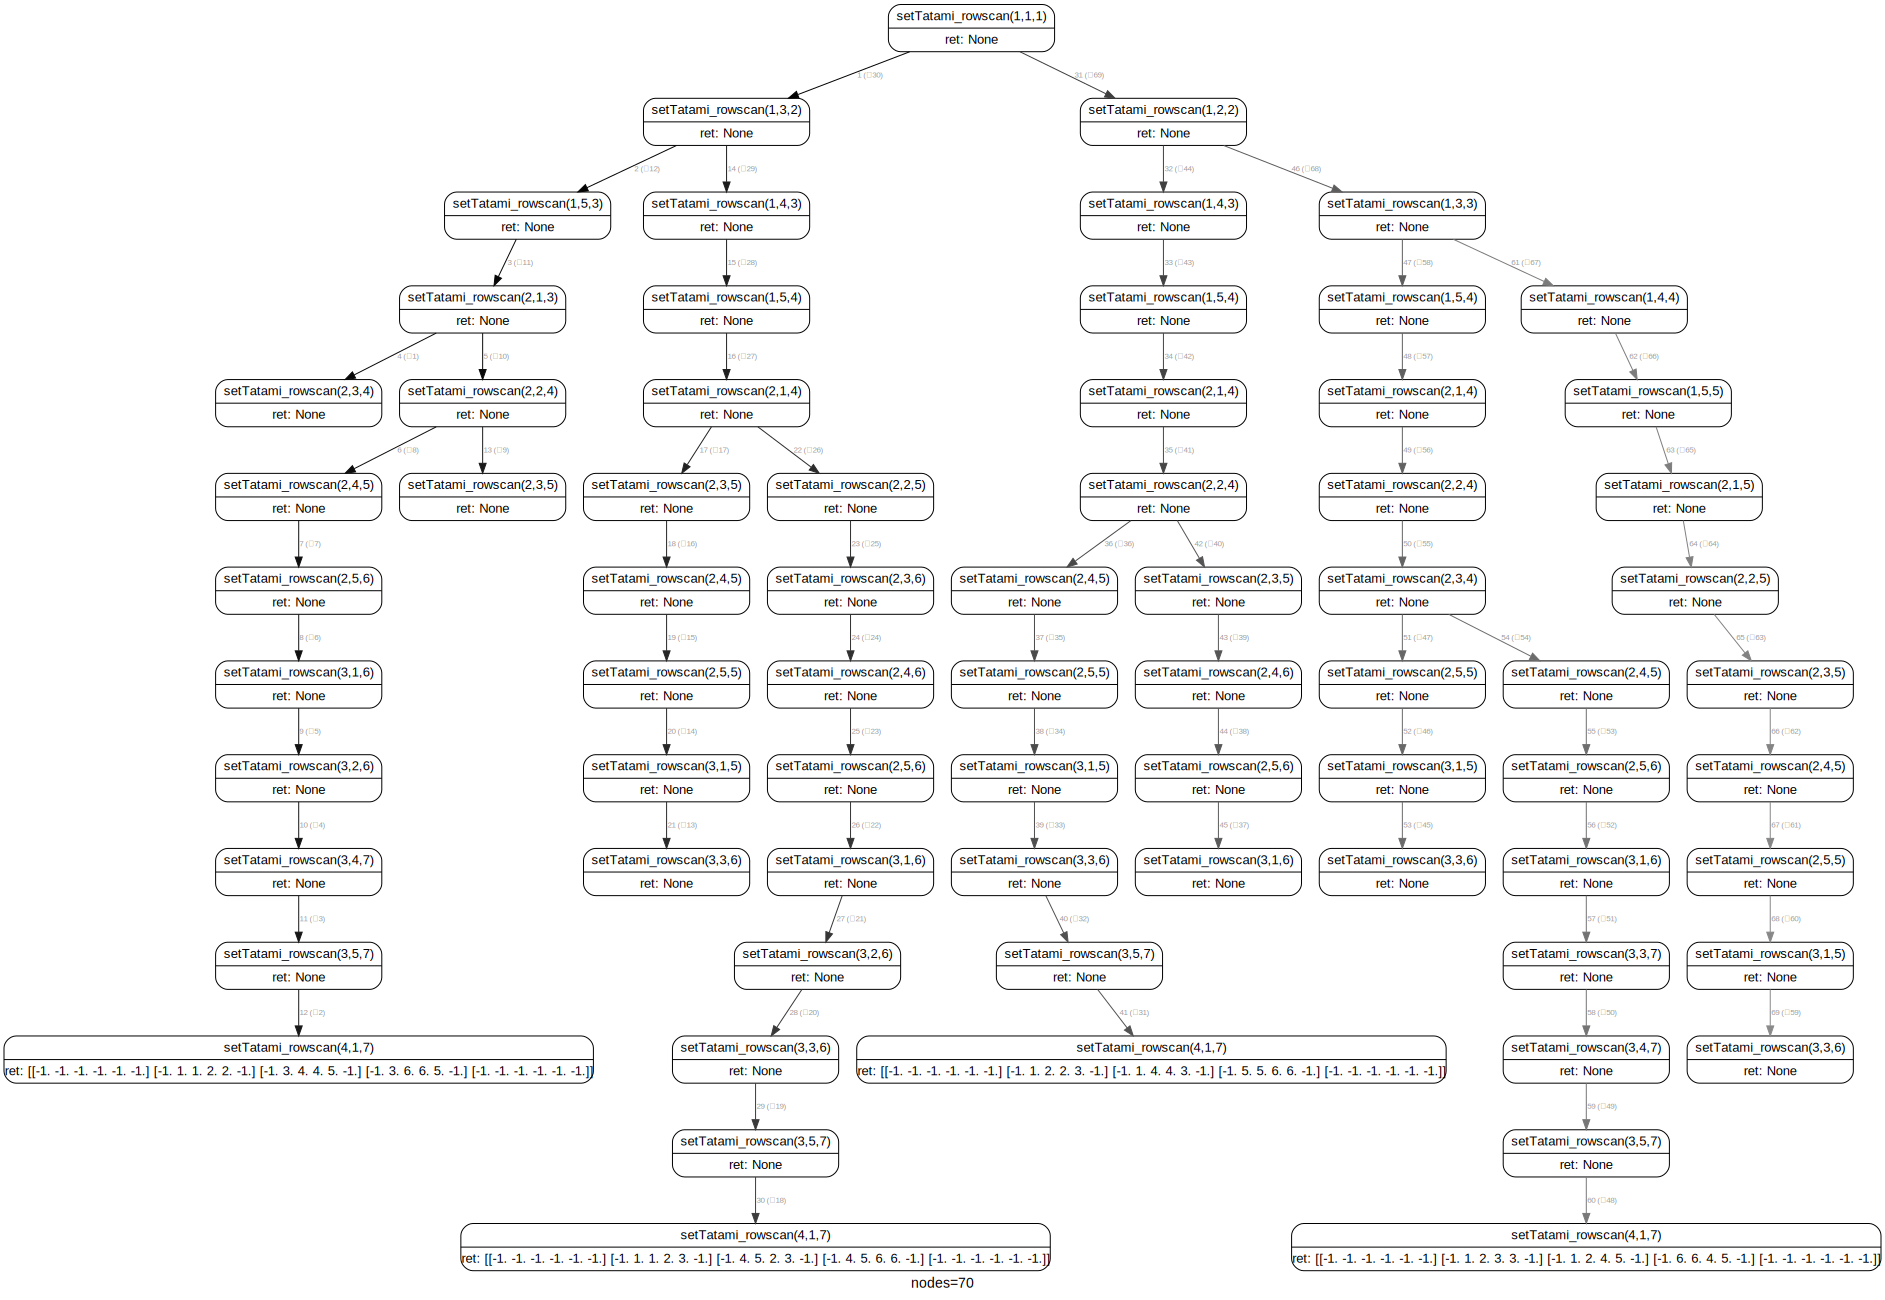
\includegraphics[width=19cm]{images/arbre4x3.pdf}
% \end{adjustwidth}
% \chapter{Tests}
% \section{Méthode et outil de test}

Les test automatisées sont réalisés à l'aide de la bibliothèque \textbf{pytest} . Les fonctions et les classes testées sont
appelées par des fonctions de test dédiées qui vérifie la concordance des valeurs retournées avec ce qui est attendu.



\section{Version Alpha}


\noindent%
\begin{adjustwidth}{-1.5cm}{0cm}

    \renewcommand{\arraystretch}{1.2}
    {\setlength{\tabcolsep}{1.5 mm}
        \begin{tabular}{|m{0.6cm}|m{5.5cm}|m{8cm}|m{2cm}|c|} \hline
            id                                                                             & Sujet                                                                                & Test d'acceptance                                                                                        & Méthode de test & Résultat \\ \hline
            518                                                                            & TACHE Utiliser la fonction pour renvoyer la réponse au gestionnaire de dojo          &
            Quand le programme est lancé et que l'utilisateur saisi comme attendu,
            une réponse lui est renvoyée dans la console                                   & Manuel                                                                               & OK                                                                                                                                    \\ \hline
            517                                                                            & TACHE Créer une fonction permettant de calculer le nombre de tatamis nécessaires
            étant donné des dimensions de dojo et qu'une solution existe                   &
            Quand la fonction est exécutée, elle retourne le nombre de tatamis nécessaires &
            Automatisé                                                                     & OK                                                                                                                                                                                                                           \\ \hline
            \multirow{3}{0.6cm}{516}                                                       & \multirow{3}{5.5cm}{TACHE Permettre au gestionnaire de dojo de poser cette question} & 1. Quand le programme est lancé, il demande a l'utilisateur la largeur du dojo                           & Automatisé      & OK       \\ \cline{3-5}
                                                                                           &                                                                                      & 2. Quand le programme est lancé, il demande a l'utilisateur la longueur du dojo                          & Automatisé      & OK       \\ \cline{3-5}
                                                                                           &                                                                                      & 3. Quand le programme est lancé, une option est disponible pour l'utilisateur pour poser cette question. & Automatisé      & OK       \\ \hline
        \end{tabular}}
\end{adjustwidth}


\noindent%
\begin{adjustwidth}{-1.5cm}{0cm}

    \renewcommand{\arraystretch}{1.2}
    {\setlength{\tabcolsep}{1.5 mm}
        \begin{tabular}{|m{0.6cm}|m{5.5cm}|m{8cm}|m{2cm}|c|} \hline
            id                       & Sujet                                                                                                                                         & Test d'acceptance                                                                                                                                                                                                          & Méthode de test & Résultat \\ \hline
            515                      & TACHE Créer une fonction permettant de calculer le nombre de tatamis nécessaires étant donné des dimensions de dojo et qu'une solution existe & Quand la fonction est executée, elle retourne le nombre de tatamis nécessaires                                                                                                                                             & Automatisé      & OK       \\ \hline

            \multirow{3}{0.6cm}{514} & \multirow{3}{5.5cm}{TACHE Permettre au gestionnaire de dojo de poser cette question}                                                          & 1. Quand le programme est lancé, il demande à l'utilisateur la largeur du dojo                                                                                                                                             & Automatisé      & OK       \\ \cline{3-5}
                                     &                                                                                                                                               & 2. Quand le programme est lancé, il demande à l'utilisateur la longueur du dojo                                                                                                                                            & Automatisé      & OK       \\ \cline{3-5}
                                     &                                                                                                                                               & 3. Quand le programme est lancé, une option est disponible pour l'utilisateur pour poser cette question.                                                                                                                   & Automatisé      & OK       \\ \hline
            \multirow{2}{0.6cm}{513} & \multirow{2}{5.5cm}{US Comprendre le nombre de dispositions possibles}                                                                        & \cellcolor{tsgrey} 1. Étant donné que l'utilisateur saisie des dimensions de dojo, quand il saisie 2, il obtient le nombre conformément à l'article de Ruskey et Woodcock de 2009                                        & Automatisé      & OK       \\ \cline{3-5}
                                     &                                                                                                                                               & \cellcolor{tsgrey} 2. Étant donné que l'utilisateur saisie des dimensions de dojo en inversant la longueur et la largeur, quand il saisie 2, il obtient le nombre conformement a l'article de Ruskey et Woodcock de 2009 & Automatisé      & OK       \\ \hline

            512                      & TACHE Utiliser la fonction pour renvoyer la réponse au gestionnaire de dojo	Alpha                                                              & Quand le programme est lancé et que l'utilisateur saisie comme attendu, une réponse lui est renvoyée dans la console                                                                                                       & Automatisé      & OK       \\ \hline
            \multirow{2}{0.6cm}{511} & \multirow{2}{5.5cm}{TACHE Demander les dimensions et permettre au gestionnaire de dojo de les saisir}                                         & 1. Quand le programme est lancée, il demande a l'utilisateur la largeur du dojo                                                                                                                                            & Automatisé      & OK       \\ \cline{3-5}
                                     &                                                                                                                                               & 2. Quand le programme est lancé, il demande a l'utilisateur la longueur du dojo                                                                                                                                            & Automatisé      & OK       \\ \hline
            \multirow{2}{0.6cm}{510} & \multirow{2}{5.5cm}{US Comprendre si une solution existe}                                                                                     & \cellcolor{tsgrey} 1. Etant donné que l'utilisateur saisie des dimensions de dojo n'ayant pas de solution, quand il saisie 1, il obtient 'Il n'existe pas de disposition possible avec des tatamis 2x1 pour ce dojo'     & Automatisé      & OK       \\ \cline{3-5}
                                     &                                                                                                                                               & \cellcolor{tsgrey} 2. Étant donné que l'utilisateur saisie des dimensions de dojo ayant au moins une disposition, quand il saisie 1, il obtient 'Il existe au moins une disposition avec des tatamis 2x1 pour ce dojo'   & Automatisé      & OK       \\ \hline
        \end{tabular}}
\end{adjustwidth}


\noindent%
\begin{adjustwidth}{-1.5cm}{0cm}

    \renewcommand{\arraystretch}{1.2}
    {\setlength{\tabcolsep}{1.5 mm}
        \begin{tabular}{|m{0.6cm}|m{5.5cm}|m{8cm}|m{2cm}|c|} \hline
            id                                                                                                       & Sujet                                                                                                                                  & Test d'acceptance                                                                                                                                                                  & Méthode de test & Résultat \\ \hline
            \multirow{2}{0.6cm}{509}                                                                                 & \multirow{2}{5.5cm}{US Créer la fonction permettant de calculer le nombre de solutions au problème étant donné les dimensions du dojo} & 1. Quand la fonction est exécutée, elle retourne le nombre de dispositions possibles conformément a l'article de Ruskey et Woodcock de 2009                                        & Automatisé      & OK       \\ \cline{3-5}
                                                                                                                     &                                                                                                                                        & 2. Quand la fonction est exécutée en inversant la longueur et la largeur, elle retourne le nombre de dispositions possibles conformément a l'article de Ruskey et Woodcock de 2009 & Automatisé      & OK       \\ \hline

            509                                                                                                      & EPIC Développer pour un gestionnaire de dojo un outil simple lui permettant de saisir les dimensions du dojo et
            de savoir si un solution existe, le nombre de tatamis nécessaires et le nombre de dispositions possibles & \cellcolor{tsgrey} cf. tests utilisateurs des US                                                                                     &                                                                                                                                                                                    &                            \\ \hline
            \multirow{2}{0.6cm}{480}                                                                                 & \multirow{2}{5.5cm}{US Calculer le nombre de tatamis nécessaires}                                                                      & 1. Étant donne que l'utilisateur saisit des dimensions de dojo avec une solution qui existe, quand il saisie 3, il obtient le nombre de tatamis nécessaires                        & Automatisé      & OK       \\ \cline{3-5}
                                                                                                                     &                                                                                                                                        & 2. Étant donne que l'utilisateur saisit des dimensions de dojo avec aucune disposition possible, quand il saisie 3, il obtient un message indiquant l'absence de solution          & Automatisé      & OK       \\ \hline
        \end{tabular}}
\end{adjustwidth}


\section{Version Beta}

\noindent%
\begin{adjustwidth}{-1.5cm}{0cm}

    \renewcommand{\arraystretch}{1.2}
    {\setlength{\tabcolsep}{1.5 mm}
        \begin{tabular}{|m{0.6cm}|m{5.5cm}|m{8cm}|m{2cm}|c|} \hline
            id                       & Sujet                                                                   & Test d'acceptance                                                                                             & Méthode de test & Résultat \\ \hline
            \multirow{2}{0.6cm}{539} & \multirow{2}{5.5cm}{TACHE Cliquer pour avoir accès aux fonctionnalités} & Quand l'application est lancée, les boutons s'affichent                                                       & Manuel          & OK       \\ \cline{3-5}
                                     &                                                                         & Quand l'utilisateur clique sur un bouton, la fonctionnalité est activée.                                      & Manuel          & OK       \\ \hline
            \multirow{3}{0.6cm}{538} & \multirow{3}{5.5cm}{TACHE Valider les dimensions}                       & Quand l'application est lancée, seules des valeurs entières peuvent être entrées                              & Manuel          & OK       \\ \cline{3-5}
                                     &                                                                         & Quand l'application est lancée, les valeurs entrables sont restreintes aux valeurs dans un intervalle défini. & Manuel          & OK       \\ \cline{3-5}
                                     &                                                                         & Quand l'utilisateur omet ou entre 0 pour au moins une dimension, un message d'erreur s'affiche.               & Manuel          & OK       \\ \hline
        \end{tabular}}
\end{adjustwidth}


\noindent%
\begin{adjustwidth}{-1.5cm}{0cm}

    \renewcommand{\arraystretch}{1.2}
    {\setlength{\tabcolsep}{1.5 mm}
        \begin{tabular}{|m{0.6cm}|m{5.5cm}|m{8cm}|m{2cm}|c|} \hline
            id                       & Sujet                                                                                           & Test d'acceptance                                                                                                                                                & Méthode de test & Résultat \\ \hline
            537                      & TACHE Offrir la possibilité d'entrer des dimensions de dojo                                     & Quand l'application est lancée, une fenêtre s'ouvre avec la possibilité d'entrer les dimensions.                                                                 & Manuel          & OK       \\ \hline
            536                      & TACHE Créer la fonction permettant d'afficher toutes les solutions                              & Quand la fonction reçoit en input les coordonnées des tatamis pour une disposition dimensions, alors elle retourne un graph avec toutes les solutions possibles" & Manuel          & OK       \\ \hline
            535                      & TACHE Créer la fonction permettant d'afficher une seule solution                                & Quand la fonction reçoit en input les coordonnées des tatamis pour une disposition dimensions, alors elle retourne un graph avec une solution possible"          & Manuel          & OK       \\ \hline
            534                      & TACHE Créer la fonction permettant de calculer les coordonnées des tatamis pour une disposition & Quand la fonction reçoit en input les dimensions d'un dojo, alors elle retourne les coordonnées des tatamis pour une disposition"                                & Manuel          & OK       \\ \hline
            533                      & TACHE Créer la fonction permettant de choisir d'afficher toutes les solutions                   & Étant donné les inputs des dimensions d'un dojo, quand cette fonction est choisie, elle retourne un graph avec toutes les solutions possibles"                   & Manuel          & OK       \\ \hline
            532                      & US Disposer d'une interface d'affichage ergonomique                                             & Quand le programme est lancé, il ouvre une interface ergonomique"                                                                                                & Manuel          & OK       \\ \hline
            531                      & TACHE Créer une classe de fenêtre type permettant d'avoir un affichage reproductible            & Quand l'application est lancée, une fenêtre s'ouvre avec les bonnes (adaptées à l'écran) et memes dimensions"                                                    & Manuel          & OK       \\ \hline
            530                      & TACHE Créer la fonction permettant de choisir d'afficher une seule solution                     & Étant donné les inputs des dimensions d'un dojo, quand cette fonction est choisie, elle retourne un graph avec une seule solution possible"                      & Manuel          & OK       \\ \hline
            \multirow{2}{0.6cm}{519} & \multirow{2}{5.5cm}{EPIC Permettre au gestionnaire de dojo de visualiser les solutions}         & cf. tests utilisateurs des US                                                                                                                                    &                 & OK       \\ \cline{3-5}
                                     &                                                                                                 & Le nombre de solution du programme donne le meme nombre de solution que le calcul de coordonnées Tatamis                                                         & Automatisé      & OK       \\ \hline
            478                      & US Afficher visuellement toutes les dispositions possibles                                      & Étant donné des dimensions d'un dojo saisies, quand il sélectionne cette option, il obtient visuellement toutes les dispositions possibles"                      & Manuel          & OK       \\ \hline
            476                      & US Afficher visuellement une disposition possible                                               & Étant donné des dimensions d'un dojo saisies, quand il sélectionne cette option, il obtient visuellement une disposition possible"                               & Manuel          & OK       \\ \hline
        \end{tabular}}
\end{adjustwidth}



\section{Version Release}

\noindent%
\begin{adjustwidth}{-1.5cm}{0cm}

    \renewcommand{\arraystretch}{1.2}
    {\setlength{\tabcolsep}{1.5 mm}
        \begin{tabular}{|m{0.6cm}|m{5.5cm}|m{8cm}|m{2cm}|c|} \hline
            id  & Sujet                                                                                                              & Test d'acceptance                                                                                                                                                                                                                  & Méthode de test & Résultat \\ \hline
            540 & EPIC Amélioration de l'expérience par ajout de fonctionnalités et amélioration de l'interface                      & \cellcolor{tsgrey}cf tests utilisateur des US                                                                                                                                                                                                        & Manuel          & OK       \\ \hline
            481 & US Affichage des dimensions sur les représentation graphiques des dispositions de tatamis                          & L'affichage graphique des solutions comprend un rappel des dimensions du dojo.                                                                                                                                                     & Manuel          & OK       \\ \hline
            482 & US Modification des dimensions du dojo                                                                             & L'application permet de saisir d'autres dimensions que celles initialement renseignées.                                                                                                                                            & Manuel          & OK       \\ \hline
            482 & US Modification des dimensions du dojo                                                                             & L'application permet de saisir d'autres dimensions que celles initialement renseignées.                                                                                                                                            & Manuel          & OK       \\ \hline
            484 & US Comprendre s'il est utile d'utiliser des demi-tatamis pour trouver une solution                                 & Si il n'existe pas de solutions avec des tatamis entiers, l'application affiche qu'il est toujours possible d'obtenir une solutions avec des demi-tatamis.                                                                         & Manuel          & OK       \\ \hline
            525 & US Obtenir une solution étant donné un nombre de tatamis                                                           & Lorsque l'utilisateur entre un nombre de tatamis, l'application propose une solution dont une des dimensions ne peut-être inférieure à 3 et dont le rapport largeur/longueur ne peut être inférieur à 1/3.& Manuel          & OK       \\ \hline
            551 & TACHE créer une fonction pour obtenir une solution étant donné un nombre de tatamis                                & Lorsque l'utilisateur entre un nombre de tatamis, l'application propose une solution dont une des dimensions ne peut-être inférieure à 3 et dont le rapport largeur/longueur ne peut être inférieur à 1/3.                         & Manuel          & OK       \\ \hline
            552 & TACHE permettre à l'utilisateur d'utiliser la fonction pour obtenir une solution étant donné un nombre de tatamis  & \cellcolor{tsgrey}La fonctionnalité est disponible sur l'interface utilisateur                                                                                                                                                                       & Manuel          & OK       \\ \hline
            527 & US calculer les dispositions pour des dimensions plus petites                                                      & \cellcolor{tsgrey} Lorsque l'utilisateur propose des dimensions, il n'existe pas de disposition aux dimensions plus grandes entre la(les) solution(s) alternative(s) proposée(s) par l'application et la demande de l'utilisateur. & Manuel          & OK       \\ \hline
            544 & TACHE créer une fonction pour calculer les dispositions pour des dimensions plus petites                           & Lorsque l'utilisateur propose des dimensions, il n'existe pas de disposition aux dimensions plus grandes entre la(les) solution(s) alternative(s) proposée(s) par l'application et la demande de l'utilisateur.                    & Automatisé      & OK       \\ \hline
            545 & TACHE permettre à l'utilisateur d'utiliser la fonction de calcul des dispositions pour des dimensions plus petites & \cellcolor{tsgrey}La fonctionnalité est disponible sur l'interface utilisateur                                                                                                                                                                       & Manuel          & OK       \\ \hline
                   \end{tabular}}
\end{adjustwidth}

\noindent%
\begin{adjustwidth}{-1.5cm}{0cm}

    \renewcommand{\arraystretch}{1.2}
    {\setlength{\tabcolsep}{1.5 mm}
        \begin{tabular}{|m{0.6cm}|m{5.5cm}|m{8cm}|m{2cm}|c|} \hline
            id  & Sujet                                                                                                              & Test d'acceptance                                                                                                                                                                                                                  & Méthode de test & Résultat \\ \hline
            541 & US Amélioration de l'expérience par ajout de fonctionnalités et amélioration de l'interface                        & \cellcolor{tsgrey}Chaque interaction proposée par l'interface correspond à une fonctionnalité bien définie et identifiable, l'interface est intuitive est agréable visuellement.                                                                     & Manuel          & OK       \\ \hline
            547 & TACHE Interface: changement de couleur de fonds                                                                    & \cellcolor{tsgrey}Test utilisateur: Le fonds de l'interface est coloré& Manuel          & OK       \\ \hline
            548 & TACHE Interface: amélioration des champs de saisie                                                                 & \cellcolor{tsgrey}Les champs de saisie sont bien identifiables& Manuel          & OK       \\ \hline
            549 & TACHE Interface: changement des couleurs et police du texte                                                        & \cellcolor{tsgrey} Le texte est coloré et avec une police lisible et moderne& Manuel          & OK       \\ \hline
            550 & TACHE Interface: redisposition et catégorisation des fonctionnalités                                               & \cellcolor{tsgrey}Les fonctionnalités sont groupées par theme sur l'interface"& Manuel          & OK       \\ \hline
            542 & US Afficher la surface                                                                                             & \cellcolor{tsgrey} La valeur d'aire affichée sur l'interface correspond à l'aire de la surface occupée par les tatamis.& Manuel          & OK       \\ \hline
        \end{tabular}}
\end{adjustwidth}

% \chapter{Gestion des versions concurrentes}

\end{document}